
\documentclass[utf8]{frontiersSCNS} % for Science, Engineering and Humanities and Social Sciences

\usepackage{url,hyperref,lineno,microtype,subcaption}
\usepackage[onehalfspacing]{setspace}
\usepackage{times}
\usepackage{pdfpages}
\usepackage{fullpage}
\usepackage{url}
\usepackage{hyperref}
\usepackage{fancyhdr}
\usepackage{graphicx}
\usepackage{tabularx}
% \usepackage{enumitem}
\usepackage{indentfirst}
\usepackage{subcaption}
\usepackage{amsmath, amssymb}

% Added by crv
\usepackage{algorithm}
\usepackage{algorithmic}
\usepackage{siunitx}
\usepackage{multirow}
% \usepackage{minitab}
\newcommand{\minitab}[2][l]{\begin{tabular}{#1}#2\end{tabular}}

% Added by bsb
\usepackage{color,soul}
\DeclareRobustCommand{\hlr}[1]{{\sethlcolor{red}\hl{#1}}}
\DeclareRobustCommand{\hlg}[1]{{\sethlcolor{green}\hl{#1}}}
\DeclareRobustCommand{\hlb}[1]{{\sethlcolor{blue}\hl{#1}}}
\DeclareRobustCommand{\hly}[1]{{\sethlcolor{yellow}\hl{#1}}}

% \linenumbers
\usepackage{natbib}


\def\keyFont{\fontsize{8}{11}\helveticabold }
\def\firstAuthorLast{Sample {et~al.}} %use et al only if is more than 1 author
\def\Authors{Woen-Sug Choi\,$^{1,*}$, Derek Olson\,$^{1}$, Duane Davis\,$^{1}$, Mabel Zhang\,$^{2}$, Bruce Allen\,$^{1}$, Andy Racson\,$^{1}$, Brian Bingham\,$^{1}$, Michael McCarrin\,$^{1}$, Carson Vogt\,$^{1}$, and Jessica Herman\,$^{1}$}

\def\Address{$^{1}$Naval Postgraduate School, $^{2}$Open Robotics}


\def\corrAuthor{Woen-Sug Choi}
\def\corrEmail{woensug.choi.ks@nps.edu}


\begin{document}
% \onecolumn
% \firstpage{1}

\title[Running Title]{Simulation of Multibeam Echosounder Perception for Underwater Manipulation} 

\author[\firstAuthorLast ]{\Authors} %This field will be automatically populated
\address{} %This field will be automatically populated
\correspondance{} %This field will be automatically populated

\extraAuth{}% If there are more than 1 corresponding author, comment this line and uncomment the next one.
%\extraAuth{corresponding Author2 \\ Laboratory X2, Institute X2, Department X2, Organization X2, Street X2, City X2 , State XX2 (only USA, Canada and Australia), Zip Code2, X2 Country X2, email2@uni2.edu}

\maketitle


\begin{abstract}
\section{}
One of the key distinguishing aspects of underwater manipulation tasks is the perception challenges of the ocean environment, specifically turbidity, backscatter, and lighting effects. Simulation of the underwater environment, while not a substitute for in-water testing, is a critical capability for developing manipulation strategies in the complex and variable ocean environment. Typically, sonar-based perception must be integrated to support manipulation planning and control. Although several approaches exist in the literature to simulate synthetic sonar images, the methods in the robotics community typically use image processing and video rendering software. In addition to a lack of physically accurate interaction model between sound and the scene of interest, several basic properties of acoustic time series are absent in these rendered sonar images—notably the point spread function of the coherent imaging system (i.e., matched filtering and beamforming), and coherent speckle. To address this deficiency, we present a beam-level time series sonar simulation method to provide raw signal data that underwater vehicle manipulator systems can exploit. A point-based scattering model is implemented to calculate the acoustic interaction between the target and environment. This is a simplified representation of target scattering, but is able to produce realistic coherent image speckle, and the correct point spread function. This model was implemented within the Gazebo framework to provide real-time scene simulations using GPU calculations. The results demonstrate that this multibeam echosounder simulator generates qualitatively realistic images with high efficiency to provide the sonar image and the physical time-series signal data. This synthetic sonar data is a key enabler for developing, testing, and evaluating underwater manipulation strategies that use sonar as a component of perception.
\tiny
 \keyFont{ \section{Keywords:} Real-time Simulation, Underwater Robotics, Multibeam Echosounder, Point Scattering Model, Gazebo Framework}
 %All article types: you may provide up to 8 keywords; at least 5 are mandatory.
\end{abstract}

\section{Introduction}
Simulation of robotic manipulation systems has proven its usability and effectiveness for designing, testing, and evaluating its capability system \citep{cook2014survey}. Especially for underwater environments, operational environments make testing the physical hardware costly and risky. It is critical to develop manipulation strategies in complex and variable ocean environments. Therefore, simulation capability to test rapidly at low cost is critical to test new designs and system control strategies from the early design stage. While simulations cannot entirely replace in-water testing, the cost of development of manipulator systems can be reduced using accurate simulators.

One of the key distinguishing aspects of underwater manipulation tasks is the perception challenges of the ocean environment, specifically turbidity, backscatter, and lighting effects. The perception simulation capability of sonar-based perception are essential for bathymetric maps or obstacle avoidance as well as to support manipulation planning and control to enable accurate feedback \citep{manhaes2016uuv}. Sonar-based perception is particularly challenging due to its physical characteristics of slow propagation speed compared to electromagnetic waves, and operation frequencies of the sonar application to model that leads to large amount of data to process requiring significant computing power to generate real-time signals with sufficient range resolutions and accuracy.

Several approaches have been developed in the literature for the open-source Gazebo robot simulator \citep{koenig04gazebo} which has emerged as a standard environment for the robotics community to simulate sonar images synthetically. In \cite{demarco15computationally} a Gazebo sonar sensor model is developed using ray tracing. The Gazebo ray-tracing functionality generates a 3D point cloud which is transformed into a sonar image. On inspection, the acoustic properties were either hard-coded or not considered and did not include speckle noise or simulation. In \cite{cerqueira17novel, cerqueira20rasterized}, a GPU-based sonar simulator is developed using rasterization. They model two types of sonar: mechanically scanned imaging sonar (MSIS) and a forward-looking sonar (FLS). The acoustic features provided in their model exploits precomputed acoustic parameters to convert the image into synthetic sonar image using geometric information of the rasterized image. The acoustic parameters to render the camera image into a sonar image includes three components: pulse distance, echo intensity, and field-of-view. 

Previous methods in the literature are based on image processing and video rendering of the simulated rays intersecting a target to convert into a sonar image pixel-wise and image-based manner \citep{demarco15computationally, cerqueira17novel, cerqueira20rasterized}. Overall, a grid is formed for the acoustic image data, and any rays that intersect a given pixel are added to it incoherently. Therefore, in addition to a lack of physically accurate interaction model between sound and the object of interest, several basic properties of pulse-echo imaging systems are absent in these rendered sonar images. Notably the point spread function of the coherent imaging system (i.e., side-lobes due to matched filtering and beamforming), and coherent speckle are absent. Speckle is the granular appearance of an image that is due to many interfering scatterers that are smaller than the resolution limit of the imaging system \citep{goodman2015statistical}. 

This study presents a beam-level time series sonar simulation method to provide a range versus intensity data, that underwater vehicle manipulator systems can exploit. A point-based scattering model is implemented, following \cite{brown17point} to calculate the interaction between sound waves and the target and environment. This is a simplified representation of target scattering, but is able to produce realistic coherent image speckle, and the correct point spread function. Also, with the underlying assumption of each beam consisting of a sum of independent scatterers on the target, this model can be easily parallelized using a GPU to provide a practical refresh rate. This model was implemented within the Gazebo framework to provide real-time scene simulations.

The application results based on proposed methods demonstrate that this multibeam echosounder simulator generates qualitatively realistic images with high efficiency to provide the sonar image and the physical time-series signal data in real-time with sufficient refresh rate showing its effectiveness and usability. This sonar data is a key enabler for developing, testing, and evaluating underwater manipulation strategies that use sonar as a perception component.

\subsection{Contribution}
The contributions of the methods in this article are to virtually produce sonar perception data with appropriate fidelity and within sufficient refresh rates. Collectively, the methods can provide physical time-series signal data to improve the simulation infrastructure that underwater manipulation strategies and systems can exploit. Individually, our contributions are as follows: 
\begin{itemize}
\item A simplified physics-based forward looking echosounder with a point-based scattering model within Gazebo framework to support underwater vehicle simulations.
\item High fidelity acoustics simulation including multibeam, scattering, noise, and target-wise reflectivity.
\item GPU parallelization for real-time sonar simulation data processing.
\end{itemize}


\section{Methods}

The model is based on a point scattering model of the echo level using the ray-based spatial discretization of the model facets as scatterers corrected with beam pattern appropriate for a line array.

\subsection{Single Beam Sonar Model}
A single sonar beam is shown in Figure \ref{fig:single_sonar_beam}. An ideal sonar beam pattern is a unit gain within the orange shaded region, and zero response outside of it. In reality, the beam response exists over all angles, although the major contribution is within the beamwidth of that particular beam. Here, a beam is modeled using discrete rays. The individual rays are indexed as $i=\{1, 2, ... N\}$ for $N$ rays and beams are indexed as $j=\{1, 2, ... N_B\}$ for $N_B$ beams.These rays correspond to intersections between the target mesh and the acoustic sensor. The following information is generated for each ray within an individual beam:

\begin{figure}[ht]
  \centering
  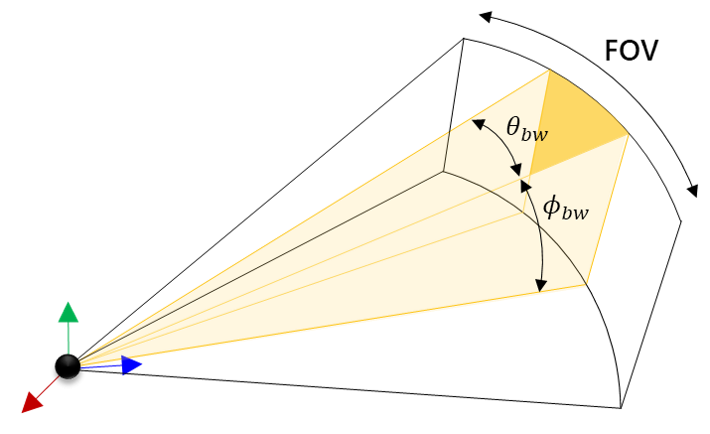
\includegraphics[width=\columnwidth]{images/single_sonar_beam.png}
  \caption{A single sonar beam with its azimuth and elevation beam widths.}
  \label{fig:single_sonar_beam}
\end{figure} 

\begin{figure}[ht]
  \centering
  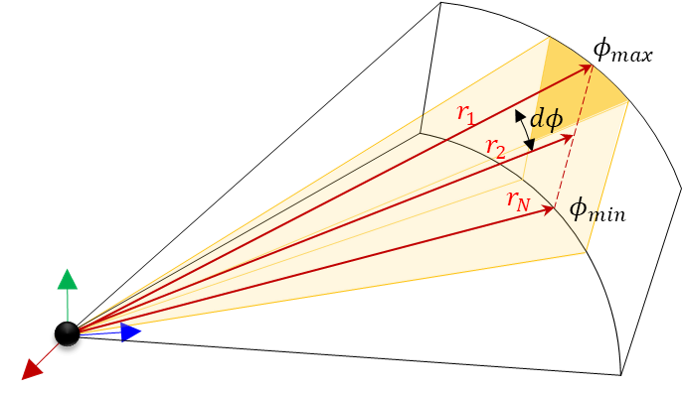
\includegraphics[width=\columnwidth]{images/rays.png}
  \caption{Set of rays forming a single sonar beam}
  \label{fig:rays}
\end{figure} 

\begin{itemize}
\item  The range $r_i$ as the distance from the origin of the sonar reference frame to the first intersection between the ray and a target in the field of view. The azimuth of the ray is fixed in the sensor frame as $\theta_i$ and the elevation angle of the ray as $\phi_i$ (Figure \ref{fig:rays})

\item  The incident angle $\alpha_i$ as the difference between the ray vector, $\mathbf{z}$, and the normal vector, $\mathbf{n}$ of the target surface at the location of intersection between the ray vector and the target surface (Figure \ref{fig:rays})

\item  The reflectivity of the target intersected by the $i$-th ray, $\mu_i$, which is a property of the target object model

\end{itemize}
This information is provided by Gazebo, and is used to calculate an acoustic time series. The range and the normal vector of the intersected target elements in the environment are obtained from the Depth-camera plugin, the generic plugin of the Gazebo. The target reflectivity is recognized using the User-camera plugin aligned with the sensor frame to convey the predefined values for each target objects spawned in the simulation environment. The methods to calculate the time series detailed below.


\subsection{Ray-based Beam Model}
We define a ray as a vector, $\mathbf{z}$, from the sensor frame origin to the first intersection with a visual object within the scene. We calculate the incident angle, $\alpha_n$, as

% \begin{equation}
%     \psi_i = cos^{-1}\left( \frac{\mathbf{z_i} \cdot \mathbf{n_i}}{\|\mathbf{z_i}\|\|\mathbf{n_i}\|} \right)
% \end{equation}
% \begin{equation}
%     \psi_i = cos^{-1}(\mathbf{\hat{z}_i} \cdot \mathbf{\hat{n}_i})
% \end{equation}
\begin{equation}
    \alpha_i = 180^{\circ} - cos^{-1}(\mathbf{\hat{z}_i} \cdot \mathbf{\hat{n}_i})
\end{equation}
where $\mathbf{\hat{z}_i}$ and $\mathbf{\hat{n}_i}$ are the ray and normal direction unit vectors respectively.

The projected ray surface area, $dA$, is the area projected onto the visual object by the individual ray as shown in Figure \ref{f:projectsurface}. If the changes in both $d\theta_i$ and $d\phi_i$ angles for each ray are assumed to be infinitesimally small, then the projected area ray scene can be calculated by

\begin{figure}[ht]
  \centering
  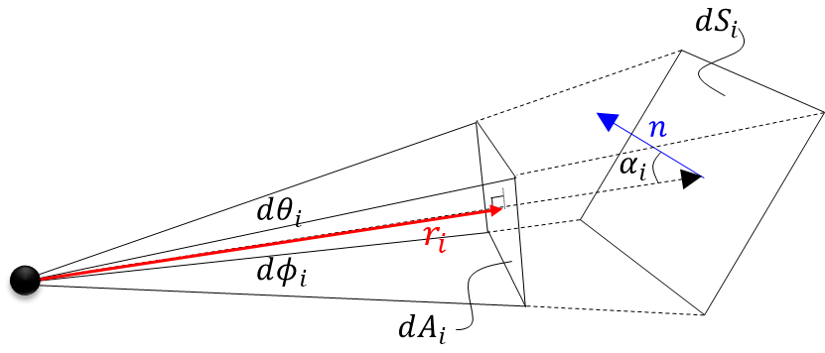
\includegraphics[width=\columnwidth]{images/sonar_surface.png}
  \caption{Projected ray surface area and surface area patch of the visual object.}
  \label{f:projectsurface}
\end{figure} 

\begin{equation}
    dA = r_i^2 d \theta_i d \phi_i
\end{equation}

Using the ray area projected onto a surface, $dS_i$ is a function of the incident angle, calculated as
\begin{equation}
    dS_i = \frac{dA}{cos(\alpha_i)}
\end{equation}
and expressed as
\begin{equation}
    dS_i = \frac{r_i^2 d \theta_i d \phi_i}{cos(\alpha_i)}
\end{equation}

The target strength is given by 
\begin{equation}
    TS_i = 10 \log\frac{I_{sca}}{I_{inc}}
\end{equation}
where $I_{sca}$ is the intensity scattered by the target measured at 1 m distance, and $I_{inc}$ is the incident intensity on the target. Models for target strength are typically complex, and depend on the shape and geometry of the target\textcolor{blue}{(DRO: cite Espana or Williams papers, perhaps Ray Lim as well)}. Since the goal of this work is to provide a realistic simulation of the geometry of a target, but not its amplitude, we use the empirical Lambert's law for scattering. This model is commonly used when the surface is very rough compared to the wavelength and represents a perfectly diffuse scattered field \textcolor{blue}{(DRO: add citations to Lambert, a few seafloor scattering papers, and optics)}. This approximation is reasonable in this case, since the sensors use a very high frequency center frequency with a wavelength on the order of O(1 mm). If a target's surface is even slightly rough, then the scattered field will be diffuse. This can occur if the target is manufactured with some surface roughness, or if it has been subject to biofouling \textcolor{blue}{(DRO add citation)}, which is very common.

Using Lambert's empirical model, the ratio of scattered to incident intensity is
\begin{equation}
    \frac{I_{ri}}{I_{Ii}} = \mu cos^2(\alpha_i)dS_i
\end{equation}
where $\mu$ is a parameter that controls the overall reflectivity to the scattered field. Substituting for $dS_i$, the intensity ratio becomes
\begin{equation}
    \frac{I_{rs}}{I_{Ii}}= \mu cos(\alpha_i)r_i^2d\theta_id\phi_i
\end{equation}
this expression is used below to calculate the amplitude of the point scatterer amplitude.

\subsubsection{Ray-based Point Scattering model}

Synthetic time series are simulated using the point-based scattering model of \cite{brown17point}. Although this model was developed for the seafloor, it can be used to characterize the incoherent field scattered by a target. It can also be adapted to generate a coherent component if that is desired as well. The model generates a spatially coherent time series that is useful in simulating narrowband sonar applications such as the FLS and MBS systems. The model uses discrete scatterers distributed over a surface defined by a discretized model mesh. These scatterers are representative of the number of surfaces a ray intersects based on the object's surface mesh. Here, we define each ray intersected surface mesh elements as scatterers; the number of rays are equivalent to number of scatterers. This approach is valid so long as the a ray intersecting surface mesh is discretized with an average ray spacing that is smaller than the resolved area of the system. If this criterion is not satisfied, then the number of rays in a beam should be increased before use in this ray-based scattering model.

The overall spectrum of the signal received from each beam, $P_j(f)$, is computed as
\begin{align}
    P_j(f) &= \frac{S(f)\sum^N_{i=1}D(\theta_{i,j},\phi_{i,j})a_{i,j}e^{iKr_{i,j}}}{r_{i,j}^2} 
    \label{e:scatteringmodel} \\
    & K = k_\omega - i\alpha_{\textrm{rad/m}} \nonumber
\end{align}

where $S(f)$ is the transmitted spectrum of the source, $N$ is the number of scatters, $a_n$ is the complex scatterer amplitude, and $f$ is the acoustic frequency. $P_j(f)$ is computed as a combination of the physical model for echo level and a complex random scale factor for speckle noise resolved in the frequency domain. The acoustic wavenumber is $k_\omega = 2\pi f/c$, where $c$ is the medium sound speed. Attenuation is included as the imaginary part of the wavenumber, $\alpha_{\textrm{rad/m}}$, with units of radians per meter. It can be related The subscript $j$ represents the index of the beams computed. A time series for each nominal beam angle is produced. The directivity pattern of beam $j$ is denoted by $D(\theta,\phi)$ and is a function of the vertical angle, $\theta$, and horizontal angle, $\phi$ between the sensor and the scatterer. The directivity function is discussed in Section \ref{s:beampattern}.

The source spectrum is a user defined input and remains constant for each ray and is modeled in the frequency domain by $S(f)$. In this model, we use a Gaussian model with a center frequency and bandwidth parameters controlling the location and width of the spectrum respectively, as in
\begin{equation}
    S(f) = S_0e^{-(f-f_c)^2b^2\pi^2} \, .
\end{equation}

The source parameter by $S_0$ and has units of \SI{}{\pascal\cdot\meter}. The decibel version of $S_0$ is the source level \citep{urick13principles}.

To obtain synthetic time series, acoustic frequency is discretized into linearly spaced vector from $f_{min}$ to $f_{max}$ and centered on the center frequency, $f_c$. The full width of the transmit spectrum is the bandwidth, $b$, a user provided input based on the sonar specifications. As an example, the bandwidth for the BlueView P900 Series FLS is \SI{2.95}{\kHz} \footnote{\url{http://www.teledynemarine.com/Lists/Downloads/p900-datasheet-hr.pdf}} \citep{blueviewp900}. The $m$-th member of the frequency vector, with $m \in [1,M]$
\begin{align}
    f_m&=m\Delta f +f_{min} \\
    f_{min} &= f_c - \frac{b}{2}\\
    \Delta f &= \frac{1}{T} \\
    M &= bT
\end{align}
where $\Delta f$ is the frequency spacing, $T$ is the desired temporal duration of the signal. The number of frequencies is $M$. The acoustic frequency vector can be mapped to the wavenumnber via $k_m = 2\pi f_m/c$. Once the frequency-domain response is calculated, then the time-domain resopnse can be computed using an inverse Fourier transform, typically implemented using the fast Fourier transform algorithm.

Spherical spreading is an appropriate assumption for modeling aoustic propagation at short ranges. The two-way transmission loss for incoherent scattering in $P_j(f)$ is captured in the denominator, $r_i^2$, where $r_i$ is the two-way distance (from source to scatterer, and back to the receiver).

The scatter amplitude, $a_i$, is calculated for each ray,
\begin{equation}
    a_i = \frac{\xi_{xi} + i \xi_{yi}}{\sqrt{2}}\sqrt{\mu_i cos^2(\alpha_i)r_i^2d\theta_id\phi_i}
\end{equation}

Although the random variable, $\xi_i$, is indexed by $i$ to represent the ray index, the real random variable and the complex random variable must both be generated and different from each other, hence the $x$ and $y$ notation. Overall, the random variables are representative of Gaussian noise and for our purposes, satisfies the speckle noise requirement \citep{brown17point}. The variables under the square root represent the target strength of an incident ray on an object.

\subsection{Directivity Pattern model}
\label{s:beampattern}
A realistic acoustic image should show the side-lobes of the beam pattern of a single point target. In some applications, it is advantageous to simulate the the time series of each element of the receive array, and perform beamforming. This method is accurate, as it reproduces the signal processing of the sonar sensor exactly. However, this approach is too computationally inefficient for real-time simulations, at least using current computing hardware. To mitigate this inefficiency, we simulate each beam assuming that the horziontal beam pattern is a uniform, ideal beam pattern within the beamwidth. The timse series are generated for a fan of beams whose directions correspond to the beamformed directions for the particular FLS or MBES.

The beam pattern of an array is defined in polar coordinates where the acoustic intensity is the distance along the radial axis and the angle is relative to the transducer axis. The beam pattern is visualized as one main lobe in the center with smaller side lobes radiating away from the main axis (Figure \ref{f:bpattern}). 

\begin{figure}[hbt!]
  \centering
  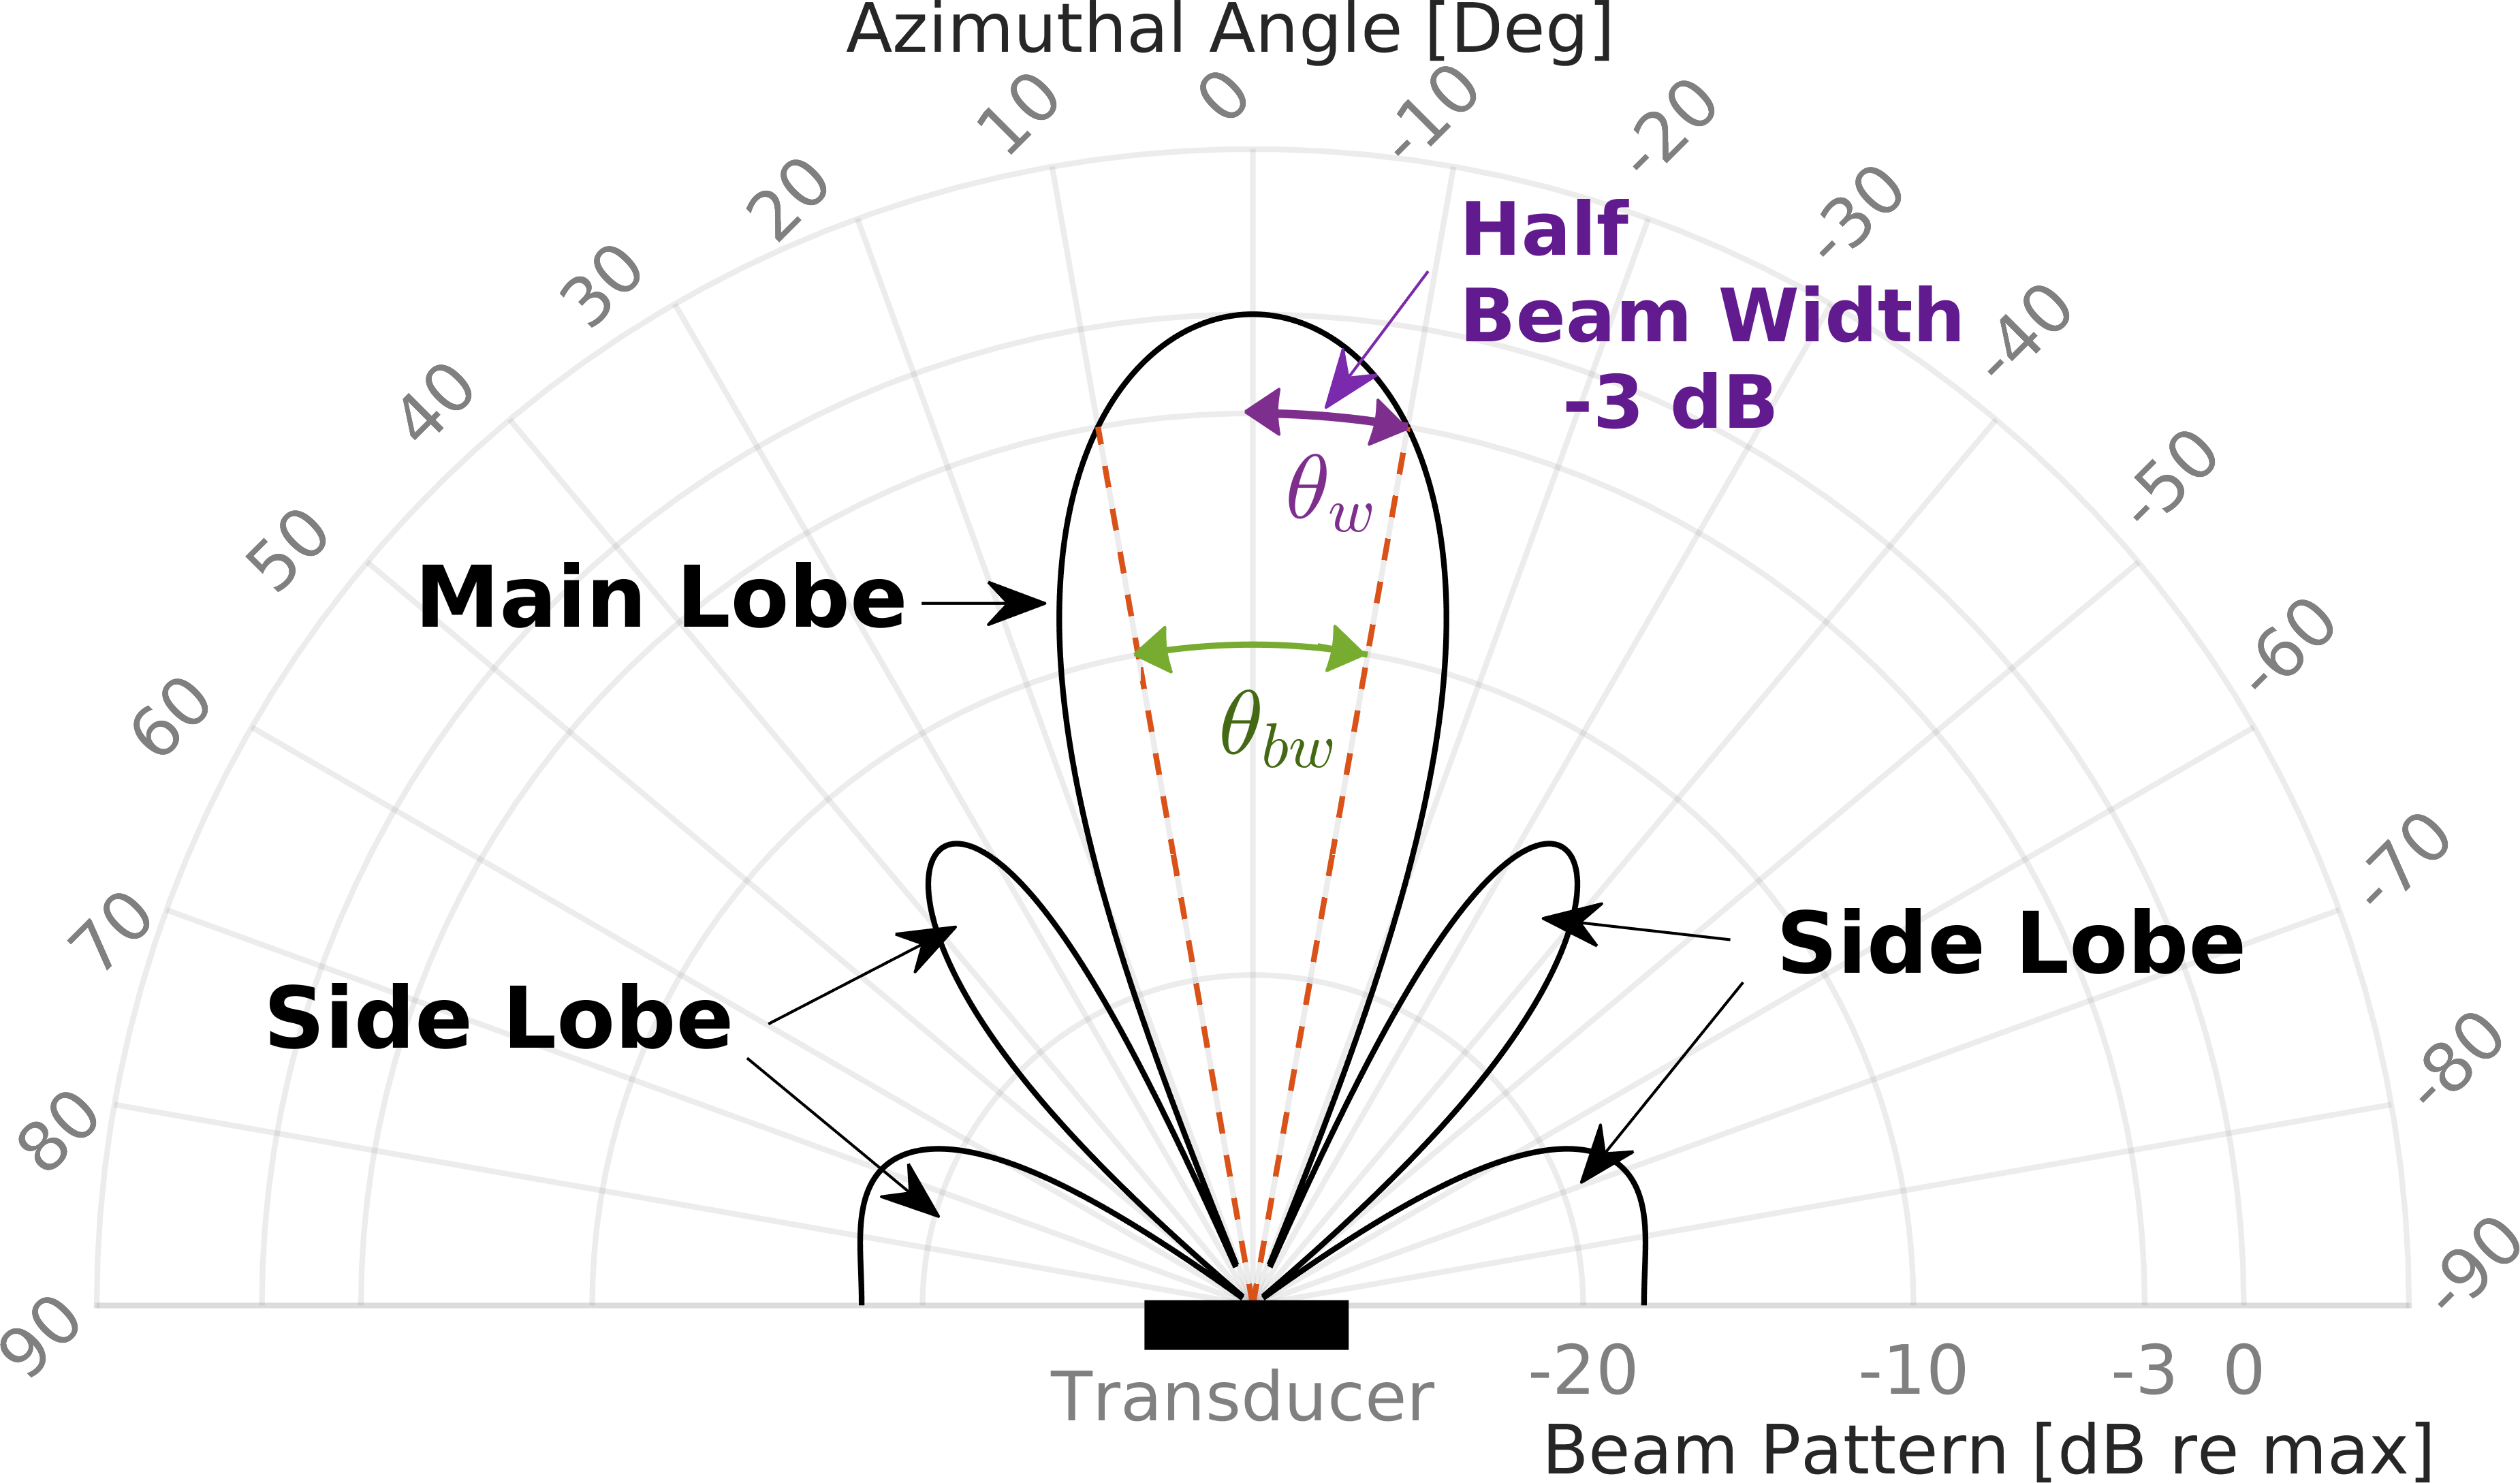
\includegraphics[width=\columnwidth]{images/beam_pattern_plot_w_annotations_mod_crop.png}
  \caption{Beam pattern schematics of half power beam width}
  \label{f:bpattern}
\end{figure}

By inspection, the highest return will be along the main axis as the response decreases off-axis. Local maxima appear away from the main axis and are referred to as side lobes. Any acoustic image or measurement will be subject to side lobes, which introduces some ambiguity into finding a target's direction in sonar data. This ambiguity is present when using any coherent imaging system that uses multiple receivers \textcolor{blue}{(DRO: add citation)}, similar to the effect of spectral leakage in spectrum estimation \textcolor{blue}{(DRO: Add citation to Harris paper on use of windows for Harmonic Analysis, Proc. IEEE)}. The sidelobe level is the decibel of ratio of the peak of the first sidelobe to the main lobe peak, and is one way of quantifying the corruption of an acoustic image due to sidelobes. Therefore, the echo intensity of a patch of a target depends on the size and position within a given beam. The beam width, $\theta_{bw}$, is marked at \SI{-3}{\decibel} on the main lobe. We define half the beam width as 
\begin{equation}
    \theta_w = \frac{\theta_{bw}}{2}
\end{equation}

The effect of side-lobes can be simulated by performing performing a correction whereby each beam is a weighted sum of all the other beams. The weight is the directivity pattern of the array with the main response axis steered in a particular direction, as in
\begin{align}
    p_{j}(t) = \frac{\sum\limits_{i=1}^{N_B}p_i(t) w_{i,j}}{\sqrt{\sum\limits_{i=1}^{N_B}|w_{i,j}|^2}}
    \label{e:beampatterneffect}
\end{align}
where $w_{i,j}$ is the weight for the $i$th beam steered in the $j$th direction. So long as the fan of beams is sampled at less than the \SI{3}{\decibel} beamwidth (ideally at least half the beamwidth), this summation reproduces the correct effect of sidelobes in the resulting time series. The form of the sum used here preserves the mean square value between the corrected pressure, and the initial simulated pressure.

The weights are the values of the beam pattern sampled at specific angles. In this work, we use the directivity pattern corresponding to a uniform linear array,
\begin{align}
    w_{ij} = B(\theta_{i} - \theta_j)
    \label{e:weights}
\end{align}
where $\theta_i$ is the horizontal angle corresponding to the $i$-th and $j$-th beam respectively. The beam pattern, $B$ is defined in the following paragraphs.

%(DRO: Put this somewhere useful) In reality, the scattered field from all locations on the target contributes to the time series for each beam, due to Huyghen's principle of wave propagation (DRO: Cite Clay and Medwin Ch 2). 
 
The beam pattern, $B(\theta)$, expresses the pressure ratio of the response of the array at an angle $\theta$, relative to the main axis.  For a continuous line array of length $L$, radiating energy at a wavelength $\lambda=2\pi/K$, the beam pattern is that of a uniform aperture function. The radiated pressure is modeled as a normalized $sinc$ function,
\begin{align}
    B(Lu)&= \textrm{sinc}(Lu) \\ 
    &= \begin{cases}
      1, & \mathrm{for}\: Lu = 0 \\
       \frac{\sin(\pi L u)}{\pi L u}, & \mathrm{otherwise} \nonumber
    \end{cases}\, ,
\end{align}
where $u$ is the electrical angle
\begin{equation}
    u = \frac{\sin(\theta)}{\lambda}
\end{equation}

The half intensity point, $\theta_w$, can be solved for by setting
\begin{equation}
    |B(\theta_w)|^2 = \left|\frac{\sin\left(\pi\frac{L}{\lambda}\sin(\theta_w)\right)}{\pi\frac{L}{\lambda}\sin(\theta_w)}\right|^2 = \frac{1}{2}    
\end{equation}

For high frequency sonar, we can assume $L \gg \lambda$, and use the small-argument approximation to the inner $\sin$ function, and $\theta_w$ becomes 
\begin{equation}
    \frac{L}{\lambda} = \frac{0.884}{\theta_{bw}} = \frac{0.442}{\theta_w}
\end{equation}

The final beam pattern is 
\begin{equation}
    B(\theta) = \frac{\sin\left(\pi\frac{0.884}{\theta_{bw}}\sin(\theta)\right)}{\pi \frac{0.884}{\theta_{bw}}sin(\theta)}
    \label{e:beampattern}
\end{equation}
Here, beam pattern, $B$, can be either positive or negative, depending on the beam angle $\theta$. When squared, it captures the intensity version of the beam pattern. 

The overall algorithm to calculate sonar model is shown in Algorithm \ref{alg}. To generate a single pair of range and intensity values for each beams, $(r_j,I_j)$ for $j$-th beam, using ray-based beam model (Equation \ref{e:scatteringmodel}), the beam pattern in Equation \ref{e:beampattern} is applied to each sampling rays. Each sample is a ray at $\phi_i$ in the range $[-\phi_w, \phi_w]$ with the associated range and intensity pair $(r_i, I_i)$. Here, $\phi_w$ is equivalent to $\theta_w$ for elevation angles. The set of ordered pairs from all rays is $i=\{1,...,N\}$ used to construct a single pair of $(r_j,I_j)$ for beam. Thereafter, for interference between beams, the Equation \ref{e:beampatterneffect} is applied with the set of pairs from all beams $j=\{1,...,N_B\}$ as a corrector.

\begin{algorithm*}
\caption{Sonar Model}
\begin{algorithmic}
\STATE $ray \leftarrow calculateRay(distance, \alpha)$
\STATE $S(f) \leftarrow calculateTransmitSpectrum(frequency)$
\FOR{$k=1:\mathrm{nBeams}$}
    \FOR{$i=1:\mathrm{nRays}$}
        \STATE $noise \leftarrow Gaussian(x,y)$
        \STATE $amplitude \leftarrow calculateAmplitude(noise, \alpha, distance, reflectivity)$
        \STATE $P(f) \leftarrow calculateReceiveSpectrum(S(f), amplitude, distance, reflectivity)$
    \ENDFOR
    \STATE $beampattern \leftarrow calculateBeamPattern(\theta)$
    \STATE $P(t) \leftarrow transformReceiveSpectrum$
\ENDFOR
\STATE $P(t)corrected \leftarrow calculateCorrectedReceiveIntensity(P(t), beampattern)$
\STATE $SPL \leftarrow calculateSoundPressureLevel(P(t)modified)$
  \label{alg}
\end{algorithmic}
\end{algorithm*}


\subsection{Gazebo and Robot Operating System (ROS) Implementation}
The Gazebo simulator and Robot Operating System (ROS) have become \emph{de facto} standards for robotic simulations. The sonar model is implemented in Gazebo as shown in Figure \ref{f:implementation}. Gazebo simulates various perception sensors using modular plugins in the environment. Based on Gazebo's camera plugin, the sonar field-of-view data is rendered from the scene using azimuth and elevation field-of-view angles of the actual sonar to generate three dimensional point clouds of the target objects. The resolutions of the point cloud is set to match with the number of beams in the sonar in azimuth angles and multiple rays in the elevation angles. Each ray in two dimensional sonar field-of-view data consists of target distance, ray angles, ray area, ray incident angle to the target, target normal, and prescribed reflectivity of the target.

Using a GPU with the NVIDIA CUDA library\footnote{\url{https://developer.nvidia.com/cuda-toolkit}} \citep{cuda}, each ray is computed in parallel using Equation \ref{e:scatteringmodel} to generate signal spectrum. Here, the complex scatter amplitudes are calculated for each ray accordingly using the sonar field-of-view data. Thereafter, ray spectra are summated to calculate the beam signal spectrum.

In order to apply beam pattern effect, the weights in Equation \ref{e:beampatterneffect} is computed. To further reduce the computation time, the calculation is also performed in matrix multiplication using the GPU with the weights (Equation \ref{e:weights}) pre-calculated when sonar rendering parameters are fixed. Finally, the Hanning window is applied and Fourier transform is performed to generate range-intensity signal data for each beam. 

The final signal data of the sonar simulation is produced in a ROS message format\footnote{\url{https://github.com/apl-ocean-engineering/hydrographic_msgs}} by \cite{acousticmsgformat} which is community-driven standardized ROS messages for hydrographic applications. The message format is designed to match that of the physical sonar applications. The final sonar signal data can be mapped onto polar coordinates to generate a sonar image.

\begin{figure*}
  \centering
  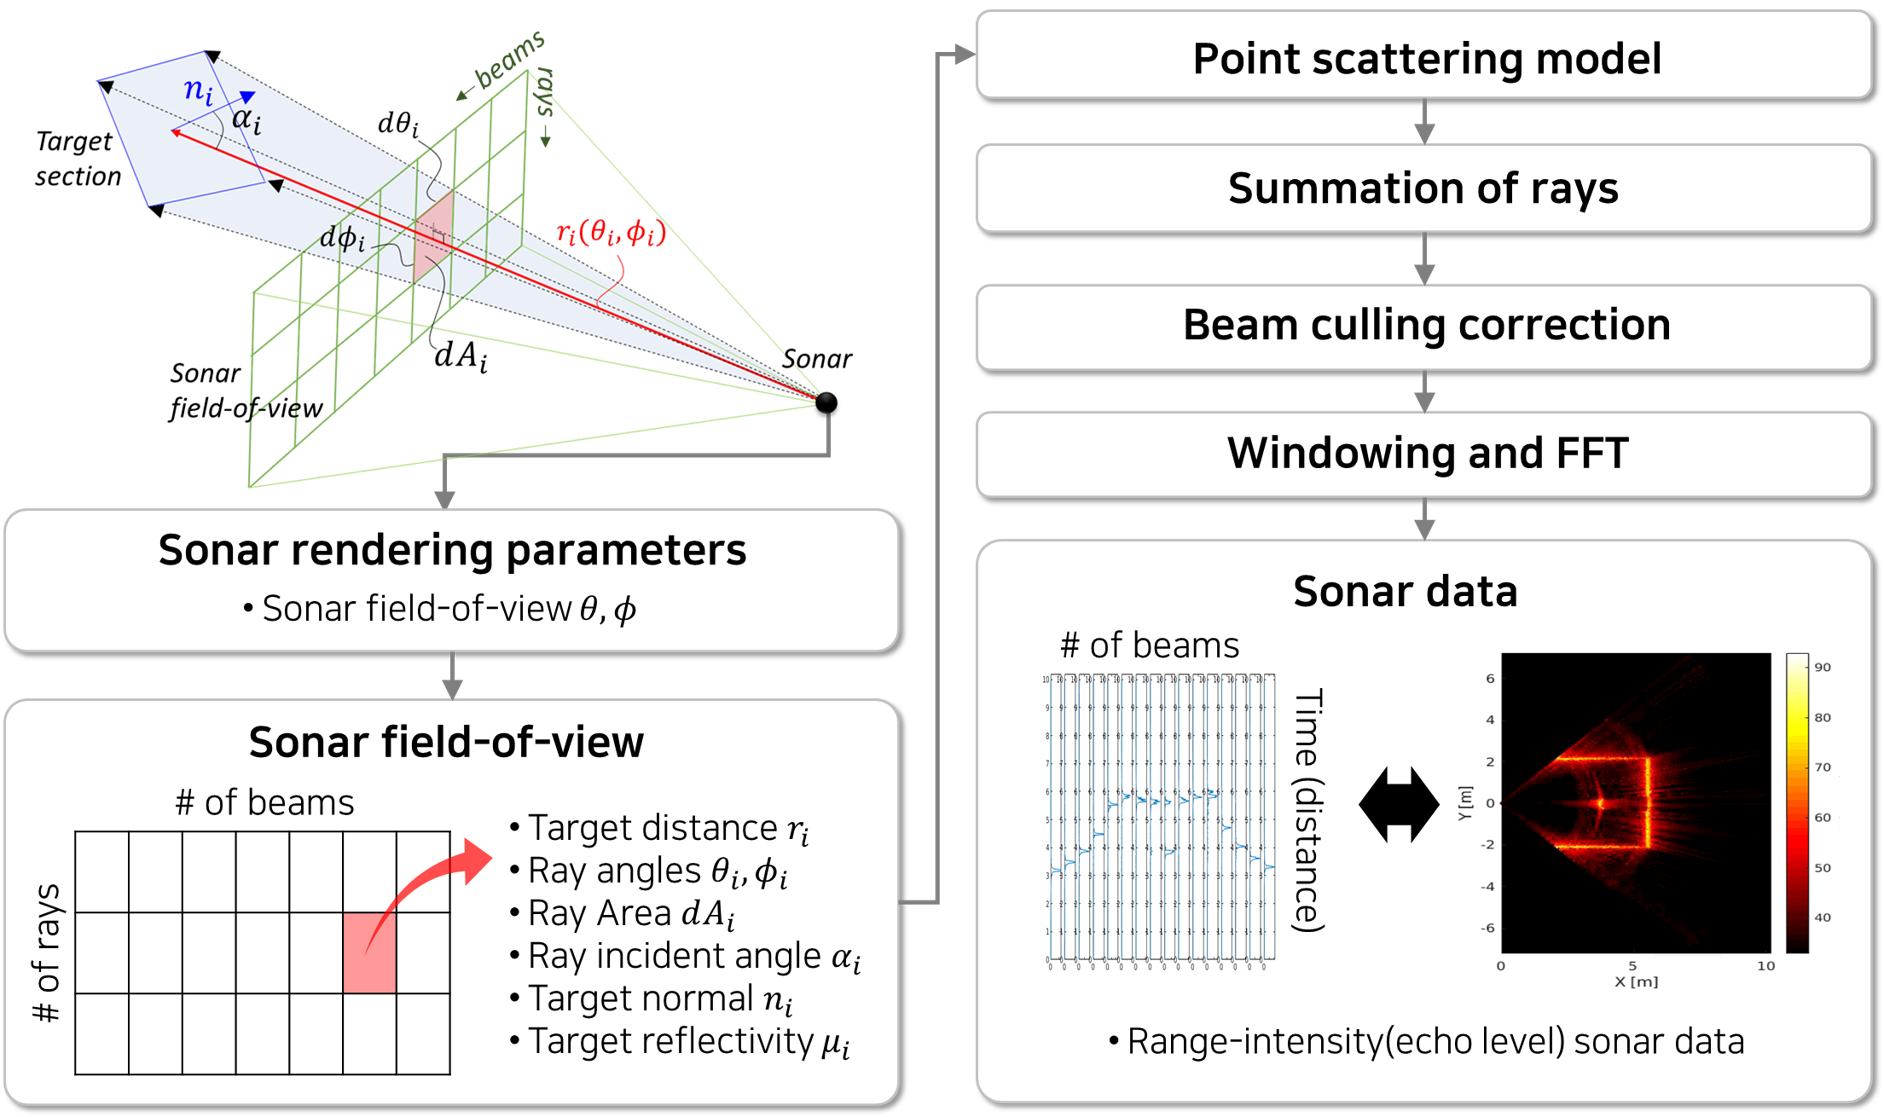
\includegraphics[width=\textwidth]{images/implementation.png}
  \caption{Overall procedures of the imaging sonar simulation process: (i) a gazebo camera plugin obtain the underwater scene; (ii) two dimensional set of sonar field-of-view data captured in the rendering scene; (iii) point scattering model is calculated for each ray data (iv) summation of rays to each beams; (v) beam pattern effect is calculated for beams; (vi) and the windowing and FFT is performed to produce range-intensity sonar data for each beams.}
  \label{f:implementation}
\end{figure*} 

\section{Real-time Multibeam Echosounder Simulation}
To evaluate our simulator, the sonar model with the developed plugin is set inside a square sonar tank with a cylinder as a target as shown in Figure \ref{f:sonar_tank_single_cylinder}. The distance between the 0.4 $m$ diameter cylinder and the sonar is 4 $m$ and the wall on the opposite side of the tank is 5.5 $m$. The sonar configurations are summarized in Table \ref{t:sonar_config}.

\begin{figure}[ht]
  \centering
  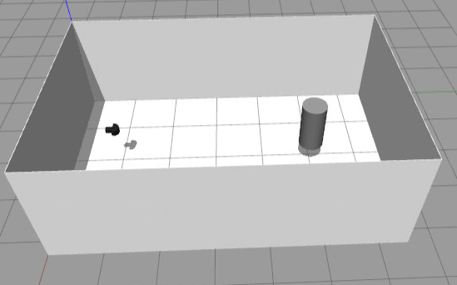
\includegraphics[width=\columnwidth]{images/single_cylinder_sonar_tank.png}
  \caption{A multibeam echosounder set in side the square sonartank with a cylinder target}
  \label{f:sonar_tank_single_cylinder}
\end{figure} 

\begin{table}[ht]
\centering
\caption{Sonar configurations}
\label{t:sonar_config}
% \resizebox{\columnwidth}{!}{%
\begin{tabular}{|ll|}
\hline
\multicolumn{2}{|l|}{\begin{tabular}[c]{@{}l@{}}Sonar configuration\\ (Blueview P900-90)\end{tabular}} \\ \hline
Frequency     & 900 \SI{}{kHz}  \\
Bandwidth     & 2.95 \SI{}{kHz}  \\
Field-of-View & 90$^\circ$ \\
Range         & 10 or 60 \SI{}{m} \\
Beam width    & 1$^\circ$ x 20$^\circ$ \\
Beam spacing  & 0.18$^\circ$ \\
\# of beams   & 512  \\
\# of rays    & 11 or 114   \\
Source level  & 220 dB re $\mu$Pa  \\ \hline
\end{tabular}
% }
\end{table}

The range-intensity sonar data obtained from the simulator is shown in Figure \ref{f:intensity_range} for 16 beams among a total of 512 beams. It shows intensity peaks at the range where the rays hit target objects in the environments. The intensity-range data can be converted into the final sonar image by mapping onto polar coordinates using azimuth and elevation angles of each beam. Figure \ref{f:single_cylindr_sonar_image} shows the live-view window in Gazebo (left) and time-averaged image colorized using MATLAB for visualization of the scattering effects. In the live-view, the data is manipulated to scale into integer format to match actual sonar data with a controllable gain. Here, both the sonar tank and the target cylinder is set to have 1e-3 reflectivity parameter value.

The result shows target object and the sonar tank in the final image. Also, the beam scattering of the signal is shown in the vicinity of the target cylinder on the colorized image. Table \ref{t:refresh_rate} shows the refresh rate of the sonar image as measured on the i9-9900K 3.6GHz, Nvidia GeForce RTX 2080Ti workstation. The most computationally demanding block is the summation that limits maximum range. If the number of rays and the maximum range are reduced, a refresh rate of above 10 Hz is achievable, providing real-time sonar data.

\begin{table}[ht]
\centering
\caption{The refresh rate and calculation time of the sonar image for various sonar configurations}
\label{t:refresh_rate}
\resizebox{\columnwidth}{!}{%
\begin{tabular}{|l|l|l|l|l|}
\hline
\multicolumn{2}{|l|}{} & \begin{tabular}[c]{@{}l@{}}Full\\ calculation\end{tabular} & \begin{tabular}[c]{@{}l@{}}Ray\\ reduced\end{tabular} & \begin{tabular}[c]{@{}l@{}}Ray/Range\\ reduced\end{tabular} \\ \hline
\multicolumn{2}{|l|}{Range {[}m{]}} & 60 & 60 & 10 \\ \hline
\multicolumn{2}{|l|}{\# of rays} & 114 & 11 & 11 \\ \hline
\multicolumn{2}{|l|}{Refresh rate {[}Hz{]}} & 0.5 & 3.0 & 10 \\ \hline
\multirow{4}{*}{\begin{tabular}[c]{@{}l@{}}Time\\ {[}s{]}\end{tabular}} & Ray signal & 0.3 & 0.02 & 0.00 \\ \cline{2-5} 
 & Summation & 1.26 & 0.16 & 0.04 \\ \cline{2-5} 
 & Correction & 0.05 & 0.05 & 0.01 \\ \cline{2-5} 
 & FFT & 0.03 & 0.03 & 0.00 \\ \hline
\end{tabular}%
}
\end{table}

\begin{figure}[ht]
  \centering
  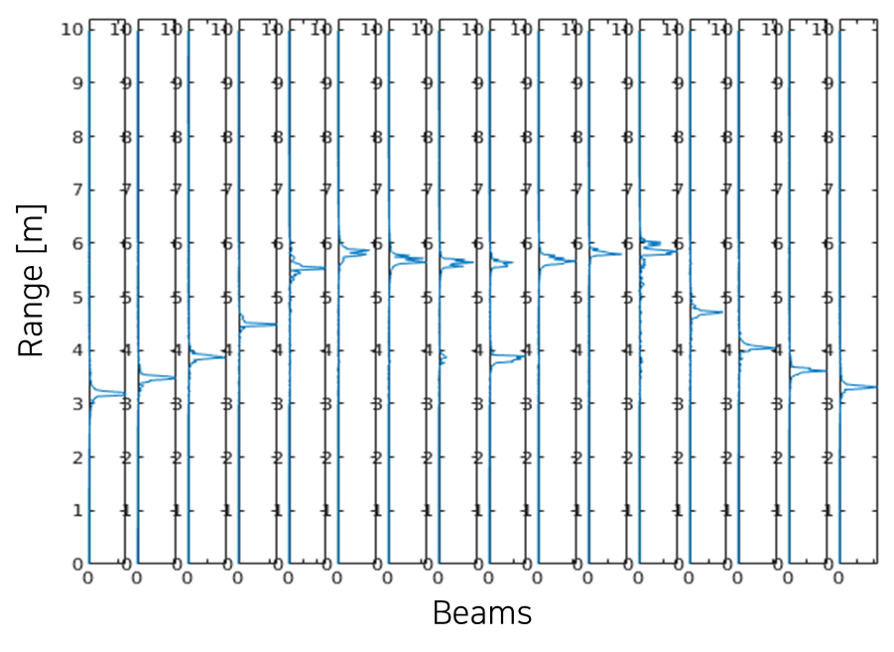
\includegraphics[width=\columnwidth]{images/intensity_range.png}
  \caption{Simulated intensity-range sonar data of a cylinder in a square sonar tank (reflectivity = 1e-3, \# of elevation rays = 11)}
  \label{f:intensity_range}
\end{figure}

\begin{figure}[ht]
  \centering
  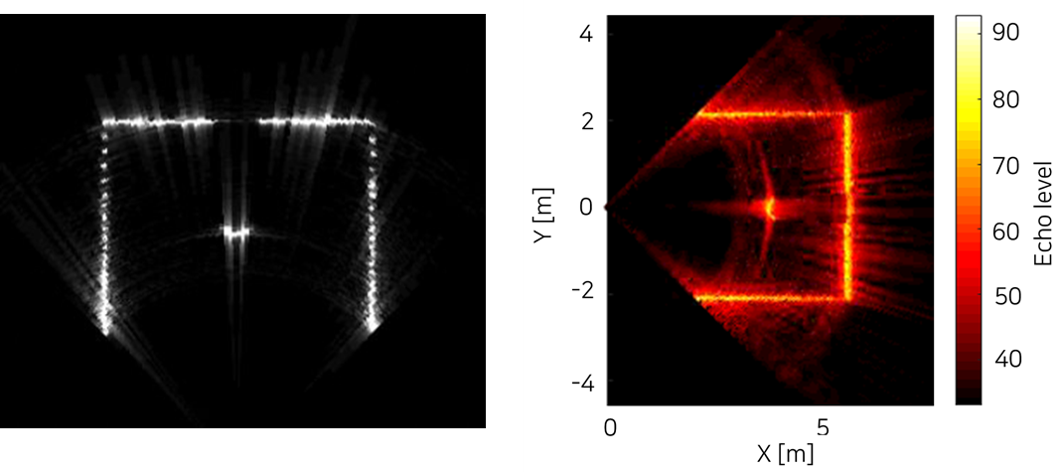
\includegraphics[width=\columnwidth]{images/single_cylinder_sonar_image.png}
  \caption{Simulated multibeam echosounder image of a cylinder in a square sonar tank with reflectivity = 1e-3 (left: live-view screenshot in the Gazebo with 11 rays, right: time-averaged image colorized using MATLAB with 114 rays).}
  \label{f:single_cylindr_sonar_image}
\end{figure}

It is often the case that the target objects in the environment have different reflectivity according to their material properties. By prescribing the reflectivity parameter for each object model in the scene, the sonar amplitude is calculated accordingly. Figure \ref{f:single_cylinder_reflectivity} shows reflectivity value set to 1e-5 for the sonar tank (left) and the target cylinder (right).

\begin{figure}[ht]
  \centering
  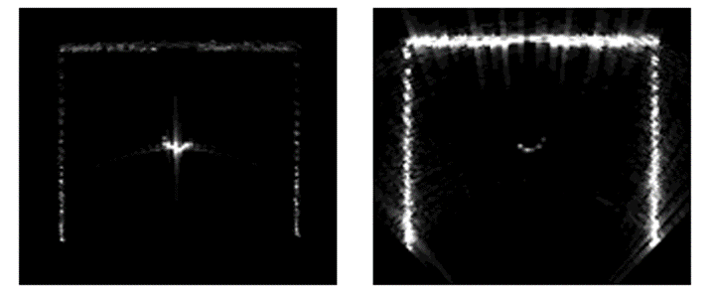
\includegraphics[width=\columnwidth]{images/single_cylinder_reflectivity.png}
  \caption{Simulated multibeam echosounder image of various reflectivities (left: low sonar tank reflectivity, right: low target cylinder reflectivity).}
  \label{f:single_cylinder_reflectivity}
\end{figure}

Figure \ref{f:two_cylinder_straight} shows two cylinders in the sonar tank. Here, the reflectivity of the sonar tank is set to 1e-4 and cylinders to 1e-2. When the two cylinders are tilted as in Figure \ref{f:two_cylinder_angled}, the amplitude gradient for the difference of distances are shown on the surface of a cylinder on the right and the difference of the incident angles on the left, as well as the blockage effect on the outer wall of the sonar tank.

\begin{figure}[t]
  \centering
  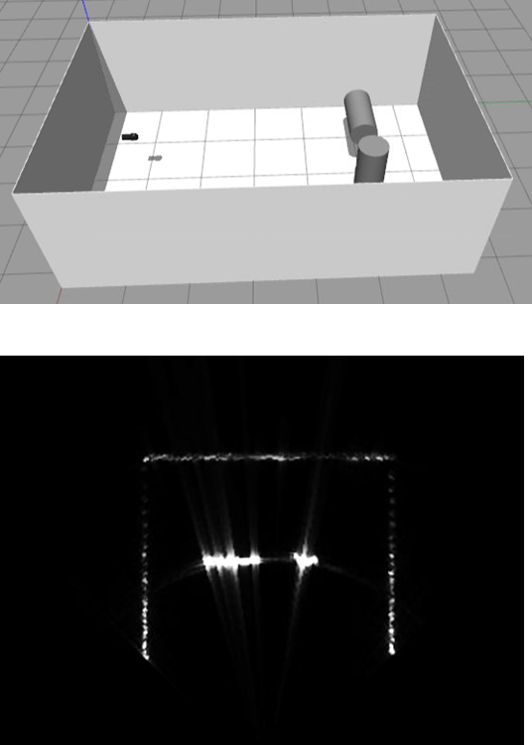
\includegraphics[width=\columnwidth]{images/two_cylinder_straight.png}
  \caption{Simulated multibeam echosounder image of two cylinder targets (top: simulation environment, bottom: live-view sonar image).}
  \label{f:two_cylinder_straight}
\end{figure} 

\begin{figure}[t]
  \centering
  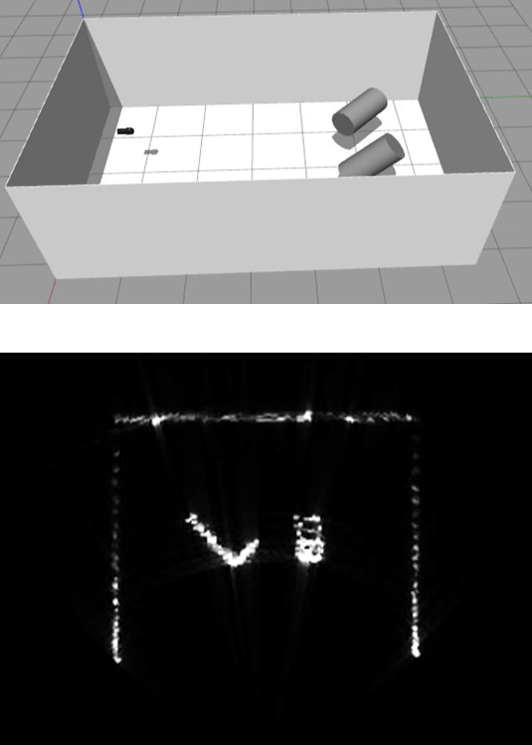
\includegraphics[width=\columnwidth]{images/two_cylinder_angled.png}
  \caption{Simulated multibeam echosounder image of two tilted cylinder targets (top: simulation environment, bottom: live-view sonar image).}
  \label{f:two_cylinder_angled}
\end{figure} 

\section{Conclusion}
In this article we have developed a method to simulate physical-based and high-fidelity multibeam echosounder perception simulation that underwater manipulation strategies and systems can exploit to include underwater acoustic perception component for development, testing and evaluation. The contributions of this research are the implementation of the point-based scattering model to represent target scattering to produce realistic coherent image speckle and the correct point spread function. Also, the usage of GPU parallelization to obtain real-time refresh rate of up to 10 Hz.

The multibeam echosounder developed can provide a sonar image and the underlying physical intensity-range time-series signal data approximate to that of a actual sonar. It is implemented as a plugin in the Gazebo framework and released as an open source project for users to manipulate for their uses. The parameterization of the plugin allows users to simulate various echosounders on the market.

\bibliographystyle{frontiersinSCNS_ENG_HUMS}
\bibliography{ocean_notes}

\end{document}
